\documentclass{beamer}  
\usetheme{Warsaw}
\usepackage{graphicx}
\title{Introduction to AI and ML}
\subtitle{ Matrix Project}
\author{A.AVINASH, EE17BTECH11005 \and \\K.DEVENDER, EE17BTECH11015}
\begin{document}

\begin{frame}

\titlepage
 
\end{frame}  

\begin{frame}[t]{Q.no.75 in JEE Mains(2010)}
If two tangents drawn from a point P to the parabola $y^{2}=4x$ are at right angles, then the locus of P is
\end{frame}

\begin{frame}
\vspace{1.5em}
Given equation of parabola is
\vspace{1.5em}
\newline
\centering
y^{2}-4x=0
\newline
\newline

Given equation in matrix form:

\[\begin{bmatrix}
x & y \\

\end{bmatrix}\begin{bmatrix}
0 & 0 \\
0 & 1
\end{bmatrix}\begin{bmatrix}
x \\
y
\end{bmatrix}+
2\begin{bmatrix}
-2 & 0 \\

\end{bmatrix}\begin{bmatrix}
x \\
y
\end{bmatrix}+0=0\]
\newline
\newline
General form of parabola is
\centering
\newline
\newline
\textbf{x}^{T}\textbf{v}\textbf{x}+2\textbf{u}^{T}\textbf{x}+F=0
\newline
\newline



\end{frame}
\begin{frame}
Comparing given equation with general form of parabola

\vspace{1.5em}

\newline
\newline
\textbf{v}=\begin{bmatrix}
0 & 0 \\
0 & 1
\end{bmatrix}
\newline
\newline
\textbf{u}^{T}=\begin{bmatrix}
-2 & 0 \\
 
\end{bmatrix}
\newline
\newline
\textbf{u}=\begin{bmatrix}
-2 \\
0 
\end{bmatrix}
\newline
\newline
F = 0

\end{frame}
\begin{frame}
\vspace{1.5em}
Let P and Q are the point of contacts of the tangents drawn on to the parabola 

\vspace{1.5em}
Then P and Q are of form $P(a^{2},2a)$ and $Q(b^{2},2b)$ 
\newline
Equation of tangent to parabola at point P is 
\newline
\[(\textbf{P}^{T}\textbf{v}+
\textbf{u}^{T})\textbf{x}+\textbf{P}^{T}\textbf{u}+
F=0\]

\newline
\newline
\[(\begin{bmatrix}
a^{2} & 2a \\
 
\end{bmatrix}\begin{bmatrix}
0 & 0 \\
0 & 1
\end{bmatrix}+
\begin{bmatrix}
-2 & 0 \\
 
\end{bmatrix})\textbf{x}+
\begin{bmatrix}
a^{2} & 2a \\
 
\end{bmatrix}\begin{bmatrix}
-2 \\
0 
\end{bmatrix}=0\]

\end{frame}
\begin{frame}

\vspace{1.5em}
\begin{bmatrix}
-2 & 2a \\
 
\end{bmatrix}\textbf{x} - 2a^{2}=0
\newline
\newline
\begin{bmatrix}
-1 & a \\
 
\end{bmatrix}\textbf{x} = a^{2} \hspace{30mm} \textbf{(1)}
\newline
\newline
\vspace{1.5em}
$Similarly, tangent at point Q is$
\newline
\newline
\begin{bmatrix}
-1 & b \\
 
\end{bmatrix}\textbf{x}=b^{2} \hspace{30mm} \textbf{(2)}
\newline
\newline
$Given two tangents are perpendicular, we have$
\begin{bmatrix}
-1 & -a \\
 
\end{bmatrix}\begin{bmatrix}
-1  \\
 b
\end{bmatrix}=0
\newline
\newline
1+ab = 0
\newline
\newline
ab = -1


\end{frame}

\begin{frame}
From above two tangent equations we have
\newline
\newline
\[\implies
\begin{bmatrix}
-1 & a  \\
-1 & b
\end{bmatrix}\textbf{x}=
\begin{bmatrix}
a^{2}  \\
b^{2}
\end{bmatrix}\]
\newline
\newline
\[\implies
\textbf{x}=
\begin{bmatrix}
-1 & a  \\
-1 & b
\end{bmatrix}^{-1}
\begin{bmatrix}
a^{2}  \\
b^{2}
\end{bmatrix}\]
\newline
\newline
\[\implies
\textbf{x}=\dfrac{1}{a-b}
\begin{bmatrix}
b & -a  \\
1 & -1
\end{bmatrix}
\begin{bmatrix}
a^{2}  \\
b^{2}
\end{bmatrix}\]
\end{frame}
\begin{frame}
\[  \implies \textbf{x}=\dfrac{1}{a-b}
\begin{bmatrix}
ab(a-b)  \\
a^{2}-b^{2}
\end{bmatrix}\]
\newline\newline
\[\implies
\textbf{x}=\begin{bmatrix}
ab  \\
a+b
\end{bmatrix}\]
\newline\newline
\[\implies
\textbf{x}=\begin{bmatrix}
-1  \\
a+b
\end{bmatrix}\]
\newline
\newline
\centering
\[\implies
   x = -1\]
\newline
\newline
x = -1 is the required locus
\end{frame}
\begin{frame}

\begin{figure}
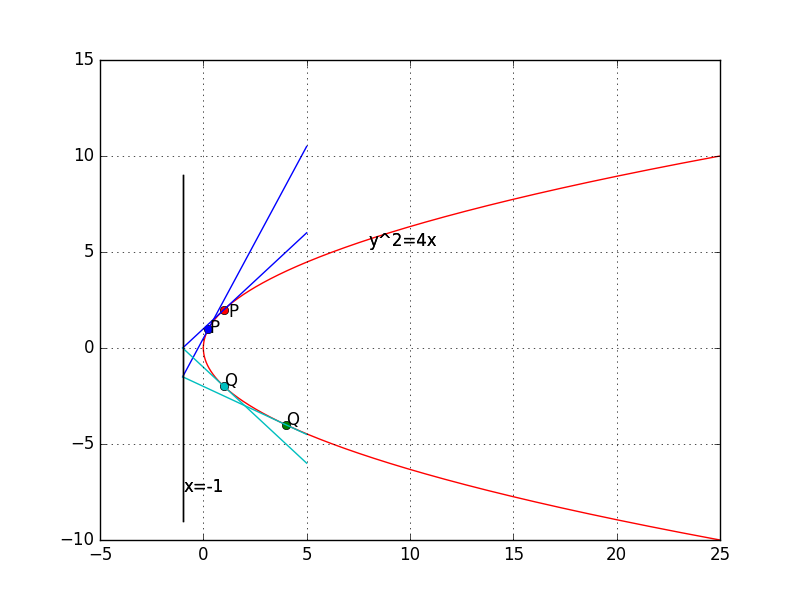
\includegraphics[width=\linewidth]{dev.png}
\end{figure}

\end{frame}
\end{document}